\chapter{Activiti BPM}\label{chp:activiti-bpm}

\section{Introdução}\label{sec:automatizacao_processos-introducao}

Criado em 2010 por ex-integrantes do projeto jBPM\cite{bpm_jbpm}, o Activiti BPM\cite{bpm_activiti} é um projeto de código aberto sob a licença Apache\cite{apache_license}, que proporciona um motor BPM leve, estável e de fácil integração. O Activiti BPM é desenvolvido na linguagem de programação Java\cite{java-history} e é facilmente integrável com aplicações existentes por sua leveza e API\cite{api} amigável, além de utilizar a notação BPMN 2.0 para a modelagem dos processos.

Neste capítulo vamos apresentar os componentes do Activiti BPM, os requisitos de software para seu funcionamento e informações sobre o ambiente de execução e modelagem do processo.

\section{Componentes}\label{sec:automatizacao_processos-gestao_processos}

O Activiti BPM é constituído por diversos componentes que possibilitam o aproveitamento do ecossistema BPM. Com exceção do \textit{Activiti Engine}, pois esse constitui o módulo principal da ferramenta, todos os demais módulos são opcionais e dependem do cenário de utilização do BPMS.

A figura \ref{fig:activiti_componentes} apresenta os componentes do Activiti BPM: \textit{Activiti Modeler}, \textit{Activiti Designer}, \textit{Activiti Kickstart}, \textit{Activiti Engine}, \textit{Activiti Explorer} e \textit{Activiti REST}. Os componentes são classificados nas categorias \textit{Modeling} (Modelagem), \textit{Runtime} (Tempo de Execução) e \textit{Management} (Gerenciamento). Esses componentes serão apresentados na seção \ref{sec:automatizacao_processos-gestao_processos_componentes} a seguir.

\begin{figure}[H]
\centering
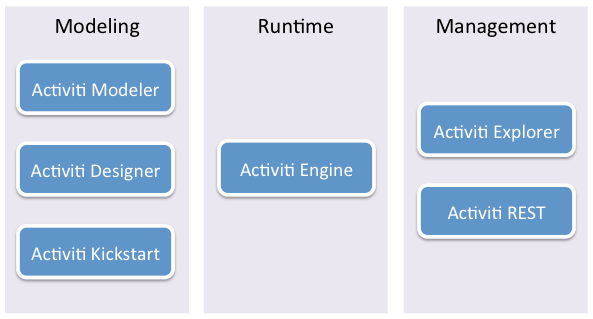
\includegraphics[width=1\textwidth]{imagens/activiti_components_overview.png}
\caption{Componentes do Activiti BPM\cite{activiti_componentes}}
\label{fig:activiti_componentes}
\end{figure}

\subsection{Activiti Engine}\label{sec:automatizacao_processos-gestao_processos_activiti_engine}

O \textit{Activiti Engine} é o componente principal, pois nele estão presentes o motor de funcionamento do BPM e as APIs para acesso e controle da ferramenta. Este componente é disponibilizado através de um simples arquivo JAR\cite{jar}, modelo de arquivo padrão para bibliotecas da linguaguem Java. Sendo assim, o motor BPM pode ser facilmente utilizado em diferentes projetos Java através da inclusão dessa biblioteca como dependência.

\subsection{Activiti Explorer}\label{sec:automatizacao_processos-gestao_processos_activiti_explorer}

O \textit{Activiti Explorer} é a interface web padrão com o usuário, disponibilizada para o controle e execução de processos. Através dessa interface, o usuário pode instalar novas definições de processos, iniciar ou cancelar processos, finalizar ou delegar tarefas. A figura \ref{fig:activiti_explorer} abaixo demonstra a lista de tarefas do Activiti Explorar disponíveis para atuação do usuário.

\begin{figure}[H]
\centering
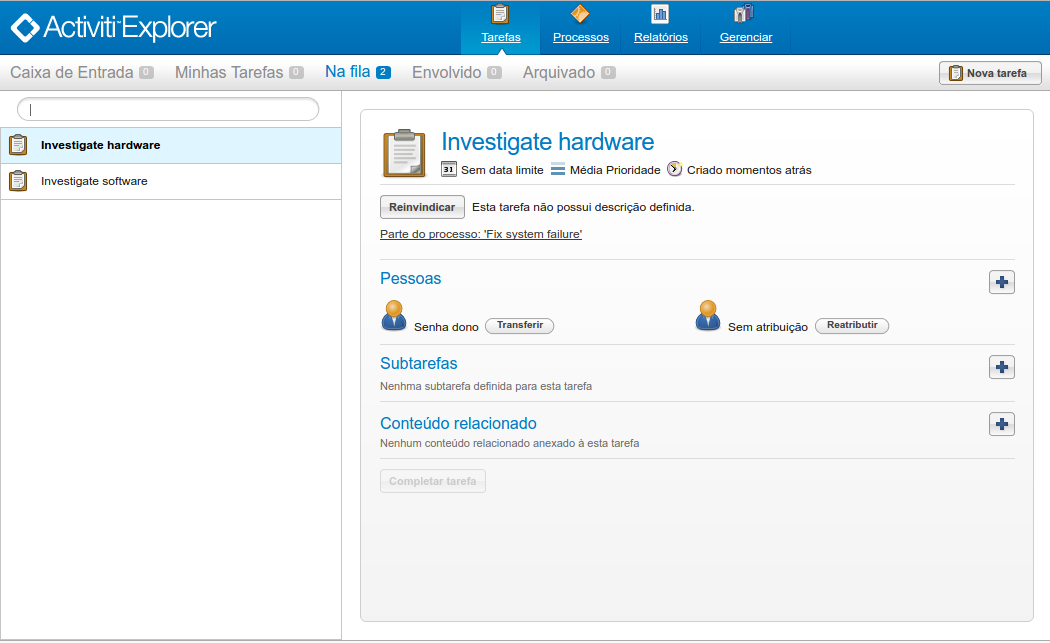
\includegraphics[width=1\textwidth]{imagens/activiti_explorer.png}
\caption{Activiti Explorer}
\label{fig:activiti_explorer}
\end{figure}

\subsection{Activiti REST}\label{sec:automatizacao_processos-gestao_processos_activiti_rest}

O \textit{Activiti REST} disponibiliza o acesso às funcionalidades principais do Activiti através de uma interface REST. Isso simplifica o acesso às suas funcionalidades por diferentes linguagens de programação e facilita a integração com diferentes aplicações de interface com o usuário, como por exemplo aplicações móveis.

\subsection{Activiti Designer}\label{sec:automatizacao_processos-gestao_processos_activiti_designer}

O \textit{Activiti Designer}, é um plugin criado para a interface de desenvolvimento Eclipse, que permite ao analista ou desenvolvedor modelar processos na notação BPMN graficamente, ao mesmo tempo em que é gerado automaticamente a notação do processo em XML. A figura \ref{fig:activiti_designer} abaixo demonstra a IDE\cite{ide} \textit{Eclipse} já com o plugin \textit{Activiti Designer} instalado para a modelagem do processo.

\begin{figure}[H]
\centering
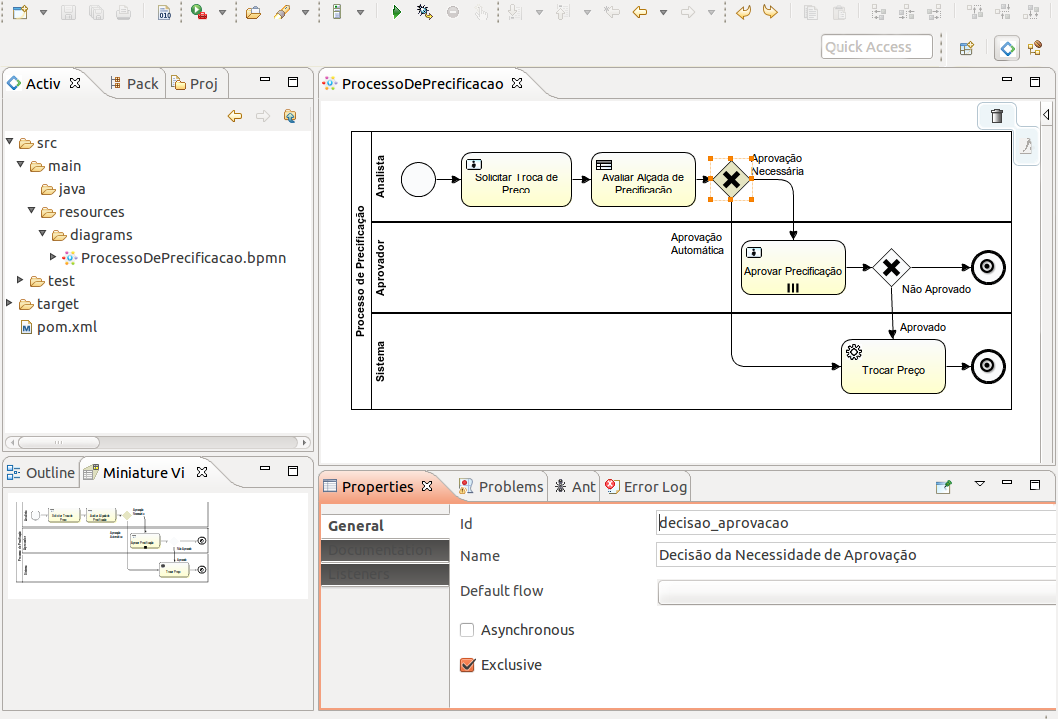
\includegraphics[width=1\textwidth]{imagens/activiti_designer.png}
\caption{Activiti Designer}
\label{fig:activiti_designer}
\end{figure}

\subsection{Activiti Modeler}\label{sec:automatizacao_processos-gestao_processos_activiti_modeler}

O \textit{Activiti Modeler} possibilita a modelagem de processos BPMN 2.0 graficamente utilizando o navegador. O Activiti Modeler já não está em desenvolvimento ativo pela equipe principal, mas permanece disponível como parte da aplicação web Activiti Explorer.

\subsection{Activiti Kickstart}\label{sec:automatizacao_processos-gestao_processos_activiti_kickstart}

O \textit{Activiti Kickstart} foi criado para facilitar a criação de processos \textit{adhoc} através de uma interface web simples e intuitiva, sem que o usuário necessite conhecer BPMN, já que são utilizados tabelas e formulários simples para a definição do fluxo de trabalho. Seu objetivo é oferecer um meio rápido para construção de processos mais simples, reduzindo assim o custo e tempo investido na automatização desses processos.

\section{Requisitos de Software}\label{sec:automatizacao_processos-requisitos}

O Activiti BPM requer um ambiente Java JDK versão 6 ou superior para seu funcionamento. Além do ambiente Java configurado, também é necessário um banco de dados para suportar a persistência das informações dos processos. Uma variedade de bancos é suportada pelo BPMS, são eles: H2\cite{db_h2}, MySQL\cite{db_mysql}, Oracle\cite{db_oracle}, PostgreSQL\cite{db_postgres}, DB2\cite{db_db2} e SQL Server\cite{db_sqlserver}.

\section{Ambiente de Execução}\label{sec:automatizacao_processos-ambiente_desenvolvimento}

Existem basicamente duas possibilidades principais para o ambiente de execução. A primeira opção é a inclusão da dependência do Activiti BPM em um projeto Java web, e o deploy do pacote WAR\cite{war} para execução em um servidor Java web. Outra opção, mais simples, é a utilização do pacote WAR já pronto para funcionamento, disponibilizado diretamente no site da ferramenta\cite{activiti_download}.

O arquivo disponibilizado no portal da ferramenta já inclui o \textit{Activiti Engine} e o \textit{Activiti Explorer} num único pacote, pré-configurados com um banco de dados em memória H2\cite{h2_inmemory} que dá suporte ao seu funcionamento e não requer nenhuma configuração adicional, já que é um banco de dados \textit{in-memory}\cite{h2_inmemory}. Para iniciar a execução do BPMS, é necessário o deploy do artefato em um servidor Java como o Apache Tomcat 7\cite{tomcat7}.

Após a instalação do artefato e inicialização do Tomcat, o portal pode ser acessado através do endereço \textit{http://127.0.0.1:8080/activiti-explorer}, dado que o Tomcat tenha sido instalado na sua configuração padrão. O usuário e senha padrão para acesso ao portal como administrador é a palavra \textit{kermit}, referência ao personagem dos Muppets\cite{kermit}. A figura \ref{fig:activiti_login} abaixo demonstra a tela de autenticação do \textit{Activiti Explorer}.

\begin{figure}[H]
\centering
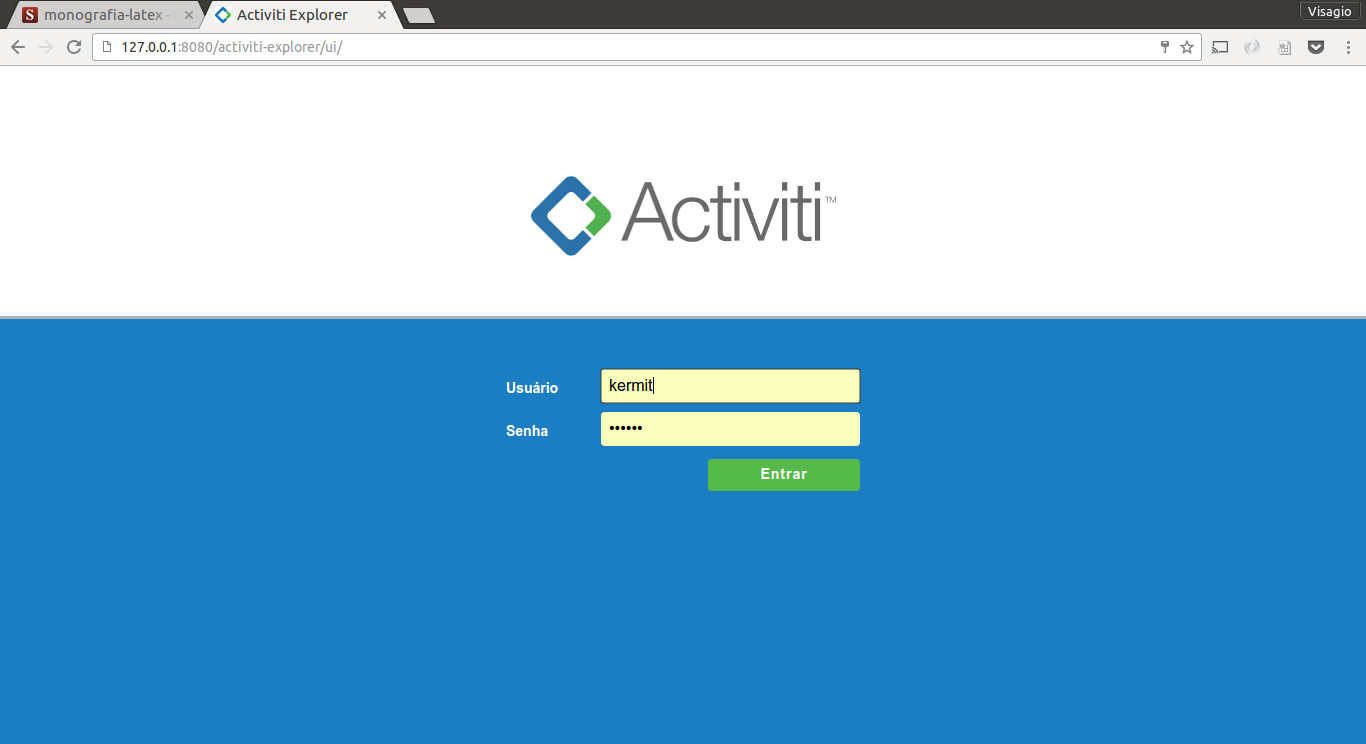
\includegraphics[width=0.9\textwidth]{imagens/activiti_login.png}
\caption{Login do Activiti Explorer}
\label{fig:activiti_login}
\end{figure}

\section{Modelagem do Processo}\label{sec:automatizacao_processos-modelagem_processo}

Para a modelagem do processo, é necessária a instalação do plugin \textit{Activiti Designer} na ferramenta de desenvolvimento \textit{Eclipse}\cite{eclipse}. Mais detalhes sobre como proceder com a instalação do plugin estão disponíveis no guia de instalação disponível no site\cite{activiti_designer}.

Ao criar um novo diagrama através da opção de criar um novo \textit{Activiti Diagram}, o \textit{Activiti Designer} cria um arquivo \textit{.bpmn} e disponibiliza duas visões para a modelagem do processo. Uma aba visual, contendo o desenho do processo, e outra aba textual, com a notação em XML. Ambas as abas estão interligadas e podem ser utilizadas para a modelagem, sendo a visual mais simples para o desenvolvimento do processo.

Para a modelagem do processo na paleta visual, é necessário arrastar os componentes visuais dispostos na aba lateral a fim de obter a modelagem desejada do processo na notação BPMN.

Ao final da modelagem, o arquivo \textit{.bpmn} é gerado para ser utilizado no \textit{deploy} do processo no motor de processos. A figura \ref{fig:processo_precificacao} representa o processo modelado na ferramenta e já descrito na notação BPMN 2.0, e o código gerado em XML pode ser consultado no apêndice \ref{code:process_bpmn}.

\begin{figure}[H]
\centering
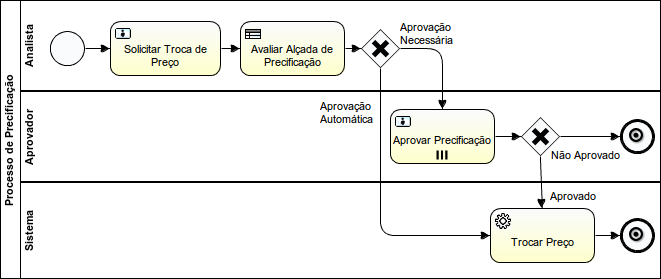
\includegraphics[width=1.0\textwidth]{imagens/ProcessoDePrecificacao}
\caption{Processo modelado no Activiti BPM}
\label{fig:processo_precificacao}
\end{figure}